\section{Architektura sieci Mask R-CNN}
\label{sec:architekrura_mask_rcnn}

Mask R-CNN rozwija się jako Mask Regions with Convolutional Neural Network (CNN) features.
Aby zrozumieć ten model, najlepiej rozważać go w kontekście ewoluowania kolejnych iteracji, którego rezultatem jest Mask R-CNN.

\subsection{Iteracja pierwsza - R-CNN}

\TODO{Tu będzie schemat R-CNN}
\TODO{Tu będzie wyjaśnienie schematu}

R-CNN, przedstawiony w 2014 roku, rozwija się jako Regions with CNN features.
Rozwiązuje zagadnienie detekcji obiektów na obrazku (to znaczy wskazuje konkretne obiekty, ale bez konkretnych pikseli).
Działanie modelu można zobrazować w następujących krokach:

\begin{enumerate}
  \item Najpierw na obszarze obrazka wejściowego generowane są tzw. propozycje regionów, przy użyciu algorytmu Selective Search\footnote{http://www.huppelen.nl/publications/selectiveSearchDraft.pdf}.
        Celem jest znalezienie regionów, w których prawdopodobnie znajduje się jakiś obiekt.
	\item Następnie, dla każdego takiego regionu wydobywane są cechy za pomocą CNN
  \item W dalszej kolejności, cechy każdego regionu analizowane są przez model Support Vector Machines (SVM).
        Wynikiem jest klasyfikacja regionu jako konkretny obiekt (lub jako brak obiektu).
	\item Na końcu, dla regionów w których wskazano obiekt następuje próba zacieśnienia obszaru regionu tak aby bardziej dopasował się do obiektu - wynikiem jest obwódka (bounding box) wskazująca położenie obiektu na obrazku
\end{enumerate}

\subsection{Iteracja druga - Fast R-CNN}

\TODO{Tu będzie schemat Fast R-CNN}
\TODO{Tu będzie wyjaśnienie schematu}

Fast R-CNN, przedstawiony w 2015 roku, usprawnia model R-CNN, w którym zidentyfikowano następujące problemy:

\begin{itemize}
	\item R-CNN składa się z czterech części:
		\begin{itemize}
			\item Selective Search do generowania regionów
			\item CNN do ekstrakcji cech
			\item SVM do klasyfikacji
			\item Model zacieśniający obwódkę
		\end{itemize}
		Sprawia to że R-CNN jest trudny do zrozumienia, problematyczny w implementacji i w wytrenowaniu.
  \item Ekstracja cech używając CNN uruchamiana jest dla każdego regionu.
        Gdy regiony zachodzą na siebie, obliczenia dla zachodzących części są powtarzane.
\end{itemize}

Fast R-CNN adresuje wyżej wymienione problemy. \\

Ekstrakcja cech przy użyciu CNN następuje tylko raz, na początku.
W ten sposób powstaje mapa cech całego obrazka.
Gdy zachodzi konieczność poznania cech regionu, zamiast liczyć cechy od nowa, wyciągany jest odpowiadający fragment mapy cech.
Metoda ta nazwana została Region of Interest Pooling.

Oprócz zmian w sposobie liczenia cech, klasyfikator SVM zastąpiono siecią neuronową.
Podobnie stało się z modelem zacieśniającym obwódkę.
Te dwie nowe sieci połączono w jedną sieć wraz z siecią CNN.
Pod-sieć klasyfikująca i pod-sieć zacieśniająca obwódke zostały włączone do sieci w sposób równoległy, to znaczy ich wyniki nie zależą od siebie nawzajem.

Zmiany te rozwiązały w dużej części problemy R-CNN wymienione wcześniej.

\subsection{Iteracja trzecia - Faster R-CNN}

\TODO{Tu będzie schemat Faster R-CNN}
\TODO{Tu będzie wyjaśnienie schematu}

Faster R-CNN, przedstawiony w 2016 roku, wprowadza kolejne usprawnienie którego zabrakło w Fast R-CNN.
Usprawnienie dotyczyło generowania regionów za pomocą algorytm Selective Search który działał wolno.
Usprawnienie polegało na zastąpieniu algorytmu nową siecią neuronową, która korzystała z cech obrazu do generowania regionów.
Jako że sieć została włączona do modelu w taki sposób, że korzystała z mapy cech które i tak była już obliczana, uzyskano szybszy model.
Dodatkowo był to kolejny krok zastępujący część modelu pod-siecią neuronową, w wyniku czego model stał się jedną siecią neuronową składającą się z pod-sieci:

\begin{itemize}
	\item Budującej mapę cech
	\item Generującej regiony
	\item Klasyfikującej
	\item Zacieśniającej obwódkę
\end{itemize}

\subsection{Iteracja czwarta - Mask R-CNN}

Schemat Mask R-CNN przedstawiony jest na rysunku \myfigref{fig:mask_r_cnn}.

\TODO{Tu będzie wyjaśnienie schematu}

Mask R-CNN, przedstawiony w 2017 roku, stanowi ostatni krok w opisanej ewolucji modelu.
Do dwóch równoległych pod-sieci - klasyfikującej oraz zacieśniającej obwódkę - wprowadza nową, równoległą pod-sieć odpowiedzialną za wskazywanie konkretnych pikseli wykrytego obiektu.

\begin{figure}[h]
  \centering
  \caption{Schemat sieci Mask R-CNN}
  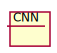
\includegraphics[width=0.5\textwidth]{mask_r-cnn.png}
  \label{fig:mask_r_cnn}
\end{figure}
